
% \section{...} 
%   \usepackage[utf8]{inputenc}
%   \usepackage[T1]{fontenc}
%   \usepackage[spanish]{babel}
%   \usepackage{amsmath}
%   \usepackage{booktabs}
%   \usepackage{multirow}
%   \usepackage{graphicx}
% Las figuras deben estar en la misma carpeta que el .tex:
%   fig_temperatura.png, fig_humedad.png, fig_velocidad.png
% ============================================================
\documentclass[11pt]{article}
\usepackage[utf8]{inputenc}
\usepackage[T1]{fontenc}
\usepackage[spanish]{babel}
\usepackage{amsmath}
\usepackage{booktabs}
\usepackage{multirow}
\usepackage{graphicx}
\usepackage[margin=2.5cm]{geometry}
% Paquetes para el diagrama de bloques (Persona 1)
\usepackage{tikz}
\usetikzlibrary{positioning, arrows.meta, babel}
% Evita el error "Incompatible glue units" de babel en español al
% escribir $60\,\%$ (el espacio antes del % ya se pone a mano).
\spanishplainpercent
% Las tablas se llaman "Tabla" en lugar de "Cuadro", como en el texto.
\addto\captionsspanish{\renewcommand{\tablename}{Tabla}}

\begin{document}

% ============================================================
% PORTADA (Persona 1)
% Los datos marcados con COMPLETAR deben llenarse en Overleaf.
% ============================================================
\begin{titlepage}
\centering
{\Large Universidad del Valle de Guatemala\par}
\vspace{0.4cm}
{\large Lógica Matemática\par}
\vspace{0.2cm}
{\large Sección XX\par} % COMPLETAR: número de sección
\vfill
{\LARGE\bfseries Sistema de control difuso para la velocidad de un ventilador\par}
\vspace{0.6cm}
{\large Aplicación de la lógica difusa\par}
\vfill
{\large\bfseries Integrantes\par}
\vspace{0.3cm}
% COMPLETAR: nombres y carnés de los integrantes
{\large
\begin{tabular}{ll}
Nombre del integrante 1 & Carné 00000 \\
Nombre del integrante 2 & Carné 00000 \\
Nombre del integrante 3 & Carné 00000 \\
Nombre del integrante 4 & Carné 00000 \\
Nombre del integrante 5 & Carné 00000 \\
\end{tabular}\par}
\vfill
{\large Catedrático: Nombre del catedrático\par} % COMPLETAR
\vspace{0.6cm}
{\large Guatemala, \today\par}
\end{titlepage}

\tableofcontents
\newpage

% ============================================================
% INTRODUCCIÓN, CONTEXTO Y OBJETIVOS (Persona 1)
% ============================================================
\section{Introducción}

En la vida diaria las personas toman decisiones a partir de descripciones imprecisas. Decimos que el día está algo caluroso, que el ambiente se siente muy húmedo o que conviene subirle un poco al ventilador, y aun así entendemos perfectamente lo que se quiere decir. La lógica clásica no se adapta bien a este tipo de razonamiento, ya que en ella una proposición solo puede ser verdadera o falsa.

La lógica difusa, propuesta por Lotfi A. Zadeh en 1965~\cite{zadeh1965}, amplía esta idea al permitir que una afirmación sea verdadera en cierto grado, expresado como un número entre 0 y 1. Gracias a esto es posible trasladar a una computadora reglas formuladas con palabras, tal como las expresaría una persona. Por esta razón la lógica difusa se ha utilizado ampliamente en el control de electrodomésticos y de sistemas de climatización, donde se busca un comportamiento suave y cercano a la intuición humana.

En este documento se aplica la lógica difusa vista en clase al diseño de un sistema que regula la velocidad de un ventilador según la temperatura y la humedad del ambiente. Se presentan el modelo del problema, la definición de las variables y sus conjuntos difusos, la base de reglas, un caso resuelto paso a paso, una simulación con distintos casos de prueba y, finalmente, las conclusiones y recomendaciones.

\subsection{Contexto del problema}

La mayoría de ventiladores domésticos funcionan con unas pocas velocidades fijas que el usuario debe seleccionar manualmente. Los modelos automáticos más sencillos utilizan un termostato con umbrales fijos: por ejemplo, el ventilador se enciende cuando la temperatura supera los $28\,^\circ$C y se apaga cuando baja de ese valor. Este enfoque tiene dos limitaciones importantes.

La primera es que produce cambios bruscos. Con $27.9\,^\circ$C el ventilador permanece apagado y con $28.1\,^\circ$C funciona a toda su capacidad, aunque una persona no percibe ninguna diferencia real entre ambas temperaturas. La segunda es que solo toma en cuenta la temperatura, cuando la sensación de calor también depende de la humedad relativa. Si el aire está muy húmedo, el sudor se evapora con más dificultad y el cuerpo se enfría menos, por lo que una misma temperatura se percibe como más incómoda.

Un controlador basado en lógica difusa permite atender ambos problemas. Por un lado, combina la temperatura y la humedad mediante reglas escritas en lenguaje cotidiano, como \emph{si la temperatura es caliente y la humedad es alta, entonces la velocidad debe ser alta}. Por otro lado, como los conjuntos difusos se traslapan, la velocidad cambia de forma gradual a medida que cambian las condiciones del ambiente. Esto resulta más cómodo para el usuario y evita que el ventilador funcione a máxima potencia cuando no es necesario.

\subsection{Objetivos}

\subsubsection*{Objetivo general}

Diseñar y analizar un sistema de control basado en lógica difusa que determine la velocidad adecuada de un ventilador a partir de la temperatura y la humedad relativa del ambiente.

\subsubsection*{Objetivos específicos}

\begin{itemize}
  \item Definir las variables de entrada y salida del sistema, junto con sus rangos, unidades y conjuntos difusos.
  \item Construir una base de reglas SI-ENTONCES que relacione las condiciones del ambiente con la velocidad del ventilador, utilizando los operadores de Zadeh.
  \item Resolver manualmente un caso numérico que muestre cada una de las etapas del proceso de inferencia.
  \item Validar el modelo mediante una simulación con varios casos de prueba y compararlo con un sistema clásico de umbrales fijos.
\end{itemize}

% ============================================================
% MARCO TEÓRICO (Persona 1)
% ============================================================
\section{Marco teórico}

\subsection{Conjuntos difusos y variables lingüísticas}

En la teoría clásica de conjuntos, un elemento pertenece o no pertenece a un conjunto, sin términos intermedios. Un conjunto difuso $A$, definido sobre un universo del discurso $X$, se describe mediante una función de pertenencia
\[
\mu_A : X \to [0, 1],
\]
que asigna a cada elemento $x$ un grado de pertenencia $\mu_A(x)$. Un valor de 0 indica que el elemento no pertenece al conjunto, un valor de 1 indica pertenencia total y los valores intermedios indican pertenencia parcial~\cite{zadeh1965}. Por ejemplo, una temperatura de $27\,^\circ$C puede considerarse templada en cierto grado y, al mismo tiempo, un poco caliente, sin que sea necesario elegir solo una de las dos opciones.

Una variable lingüística es aquella cuyos valores son palabras en lugar de números. En este proyecto la temperatura puede tomar los valores \emph{fría}, \emph{templada} y \emph{caliente}, y cada uno de ellos se representa con un conjunto difuso sobre el rango de temperaturas considerado. Esto permite describir el comportamiento del sistema con el mismo vocabulario que usaría una persona.

\subsection{Operadores de Zadeh}

Para combinar grados de pertenencia se utilizan los operadores propuestos por Zadeh, que generalizan las operaciones de la lógica clásica:
\begin{align*}
\text{Conjunción (Y):} \quad & \mu_{A \cap B}(x) = \min\{\mu_A(x), \mu_B(x)\}, \\
\text{Disyunción (O):} \quad & \mu_{A \cup B}(x) = \max\{\mu_A(x), \mu_B(x)\}, \\
\text{Negación (NO):} \quad & \mu_{\bar{A}}(x) = 1 - \mu_A(x).
\end{align*}
Cuando los grados de pertenencia son únicamente 0 o 1, estos operadores producen los mismos resultados que la lógica clásica, por lo que esta puede verse como un caso particular de la lógica difusa.

\subsection{Reglas difusas}

El conocimiento del sistema se expresa mediante reglas de la forma
\begin{center}
SI $x$ es $A$ Y $y$ es $B$, ENTONCES $z$ es $C$,
\end{center}
donde la parte del SI se llama antecedente y la parte del ENTONCES se llama consecuente. Desde el punto de vista lógico, cada una de estas reglas corresponde a una cláusula de Horn, ya que reúne varias condiciones y tiene una única conclusión. A diferencia de la lógica clásica, una regla difusa no necesita cumplirse por completo para tener efecto: se activa en el mismo grado en que se cumple su antecedente. A ese valor se le llama fuerza de activación de la regla.

\subsection{Inferencia de Mamdani y defuzzificación}

El método de inferencia más utilizado en problemas de control es el propuesto por Mamdani y Assilian~\cite{mamdani1975}. Este método toma valores numéricos de entrada y los procesa en cuatro etapas: fuzzificación, evaluación de reglas, agregación y defuzzificación. En la evaluación de reglas, el conjunto difuso del consecuente de cada regla se recorta a la altura de su fuerza de activación mediante el operador mínimo. En la agregación, los conjuntos recortados de todas las reglas se combinan con el operador máximo para formar un único conjunto difuso de salida.

Por último, la defuzzificación convierte ese conjunto en un solo número que puede aplicarse al sistema real. El método más común es el del centroide, que calcula el centro de gravedad del área bajo el conjunto de salida:
\[
z^{*} = \frac{\int z \, \mu(z) \, dz}{\int \mu(z) \, dz}.
\]
De forma intuitiva, $z^{*}$ es el punto en el que la figura formada por el conjunto de salida quedaría en equilibrio si se apoyara sobre él. Cuando el cálculo se hace a mano o en una computadora, las integrales suelen aproximarse con sumas sobre un conjunto de puntos del universo de salida.

% ============================================================
% DESCRIPCIÓN GENERAL DEL SISTEMA Y DIAGRAMA DE BLOQUES (Persona 1)
% ============================================================
\section{Descripción general del sistema}

El sistema propuesto recibe dos mediciones del ambiente, la temperatura en grados Celsius y la humedad relativa en porcentaje, y entrega un solo valor: la velocidad a la que debe girar el ventilador, expresada como porcentaje de su velocidad máxima. Tanto las entradas como la salida son valores numéricos exactos, que en lógica difusa se conocen como valores \emph{crisp}. Entre la entrada y la salida, la información pasa por las etapas del método de Mamdani descritas en la sección anterior, como se muestra en el siguiente diagrama de bloques.

\begin{center}
\begin{minipage}{\textwidth}
\centering
\begin{tikzpicture}[
  node distance=0.55cm,
  etapa/.style={rectangle, rounded corners=3pt, draw=blue!60!black, fill=blue!8,
                thick, text width=5.6cm, minimum height=0.9cm, align=center,
                font=\small},
  extremo/.style={rectangle, draw=black!70, fill=black!8, thick,
                  text width=5.6cm, minimum height=0.9cm, align=center,
                  font=\small},
  conocimiento/.style={rectangle, draw=black!60, dashed, text width=3cm,
                       minimum height=1cm, align=center, font=\footnotesize},
  flecha/.style={-{Stealth[length=2.5mm]}, thick},
  apoyo/.style={-{Stealth[length=2mm]}, dashed, black!60},
  etiqueta/.style={right, font=\footnotesize\itshape, text=black!70}
]
  % Flujo principal
  \node[extremo] (entrada) {\textbf{Entradas crisp}\\ Temperatura ($^\circ$C) y humedad (\%)};
  \node[etapa, below=of entrada] (fuzz) {\textbf{Fuzzificación}};
  \node[etapa, below=of fuzz] (reglas) {\textbf{Evaluación de reglas}\\ (inferencia)};
  \node[etapa, below=of reglas] (agreg) {\textbf{Agregación}\\ (operador máximo)};
  \node[etapa, below=of agreg] (defuzz) {\textbf{Defuzzificación}\\ (método del centroide)};
  \node[extremo, below=of defuzz] (salida) {\textbf{Salida crisp}\\ Velocidad del ventilador (\%)};

  \draw[flecha] (entrada) -- node[etiqueta] {valores medidos} (fuzz);
  \draw[flecha] (fuzz) -- node[etiqueta] {grados de pertenencia} (reglas);
  \draw[flecha] (reglas) -- node[etiqueta] {conjuntos de salida recortados} (agreg);
  \draw[flecha] (agreg) -- node[etiqueta] {conjunto difuso de salida} (defuzz);
  \draw[flecha] (defuzz) -- node[etiqueta] {valor numérico único} (salida);

  % Base de conocimiento
  \node[conocimiento, left=1.2cm of fuzz] (fp) {Funciones de pertenencia};
  \node[conocimiento, left=1.2cm of reglas] (br) {Base de reglas SI-ENTONCES};
  \draw[apoyo] (fp) -- (fuzz);
  \draw[apoyo] (br) -- (reglas);
\end{tikzpicture}\par
\small Diagrama de bloques del sistema de control difuso.
\end{minipage}
\end{center}

A continuación se describe la función de cada bloque:
\begin{enumerate}
  \item \textbf{Entradas crisp.} Son los valores medidos por los sensores, por ejemplo $28\,^\circ$C de temperatura y $60\,\%$ de humedad relativa.
  \item \textbf{Fuzzificación.} Cada entrada se evalúa en las funciones de pertenencia de su variable. La temperatura se traduce en grados de pertenencia a los conjuntos Fría, Templada y Caliente, y la humedad en grados de pertenencia a los conjuntos Baja, Media y Alta.
  \item \textbf{Evaluación de reglas.} Con los grados obtenidos se evalúa cada regla de la base de reglas. La fuerza de activación de cada una se calcula con los operadores de Zadeh, y el conjunto de velocidad de su consecuente (Baja, Media o Alta) se recorta a esa altura.
  \item \textbf{Agregación.} Los conjuntos recortados de todas las reglas se combinan con el operador máximo. El resultado es un único conjunto difuso que resume la recomendación de todas las reglas.
  \item \textbf{Defuzzificación.} Mediante el método del centroide, el conjunto agregado se convierte en un solo número.
  \item \textbf{Salida crisp.} Es la velocidad final del ventilador, un valor entre 0 y $100\,\%$ que se envía al motor.
\end{enumerate}

Las funciones de pertenencia y la base de reglas forman la base de conocimiento del sistema. Las primeras se detallan en la siguiente sección y la segunda en la Sección~\ref{sec:reglas}.

\section{Definición de variables, fuzzificación y conjuntos difusos}

\subsection{Variables del sistema}

El sistema de control difuso del ventilador cuenta con dos variables de entrada y una de salida. La Tabla~\ref{tab:variables} resume sus universos del discurso, unidades y conjuntos difusos.

\begin{table}[h]
\centering
\caption{Variables de entrada y salida del sistema.}
\label{tab:variables}
\begin{tabular}{llcp{2.6cm}l}
\toprule
\textbf{Variable} & \textbf{Tipo} & \textbf{Universo} & \textbf{Unidad} & \textbf{Conjuntos difusos} \\
\midrule
Temperatura & Entrada & $[10, 40]$ & $^\circ$C & Fría, Templada, Caliente \\
Humedad relativa & Entrada & $[0, 100]$ & \% & Baja, Media, Alta \\
Velocidad del ventilador & Salida & $[0, 100]$ & \% de la velocidad máxima & Baja, Media, Alta \\
\bottomrule
\end{tabular}
\end{table}

\subsection{Funciones de pertenencia}

Se utilizaron funciones trapezoidales y triangulares. La función trapezoidal con parámetros $(a, b, c, d)$ se define como:
\[
\mu(x) =
\begin{cases}
0, & x \le a \ \text{ o } \ x \ge d, \\[4pt]
\dfrac{x - a}{b - a}, & a < x < b, \\[8pt]
1, & b \le x \le c, \\[4pt]
\dfrac{d - x}{d - c}, & c < x < d.
\end{cases}
\]

La función triangular $(a, b, c)$ es el caso particular en que $b = c$. En los conjuntos de los extremos se cumple $a = b$ o $c = d$, por lo que tienen una sola pendiente. Los parámetros de cada conjunto se muestran en la Tabla~\ref{tab:parametros}.

\begin{table}[h]
\centering
\caption{Parámetros de las funciones de pertenencia.}
\label{tab:parametros}
\begin{tabular}{llcc}
\toprule
\textbf{Variable} & \textbf{Conjunto} & \textbf{Tipo} & \textbf{Parámetros} \\
\midrule
\multirow{3}{*}{Temperatura ($^\circ$C)} & Fría & Trapecio & $(10, 10, 16, 22)$ \\
 & Templada & Triángulo & $(18, 24, 30)$ \\
 & Caliente & Trapecio & $(26, 32, 40, 40)$ \\
\midrule
\multirow{3}{*}{Humedad (\%)} & Baja & Trapecio & $(0, 0, 25, 50)$ \\
 & Media & Triángulo & $(30, 50, 70)$ \\
 & Alta & Trapecio & $(50, 75, 100, 100)$ \\
\midrule
\multirow{3}{*}{Velocidad (\%)} & Baja & Trapecio & $(0, 0, 20, 45)$ \\
 & Media & Triángulo & $(30, 50, 70)$ \\
 & Alta & Trapecio & $(55, 80, 100, 100)$ \\
\bottomrule
\end{tabular}
\end{table}

Las Figuras 1, 2 y 3 muestran las funciones de pertenencia de cada variable. En las dos primeras se marcan los valores de ejemplo usados en la siguiente subsección.

\begin{center}
\begin{minipage}{\textwidth}
\centering
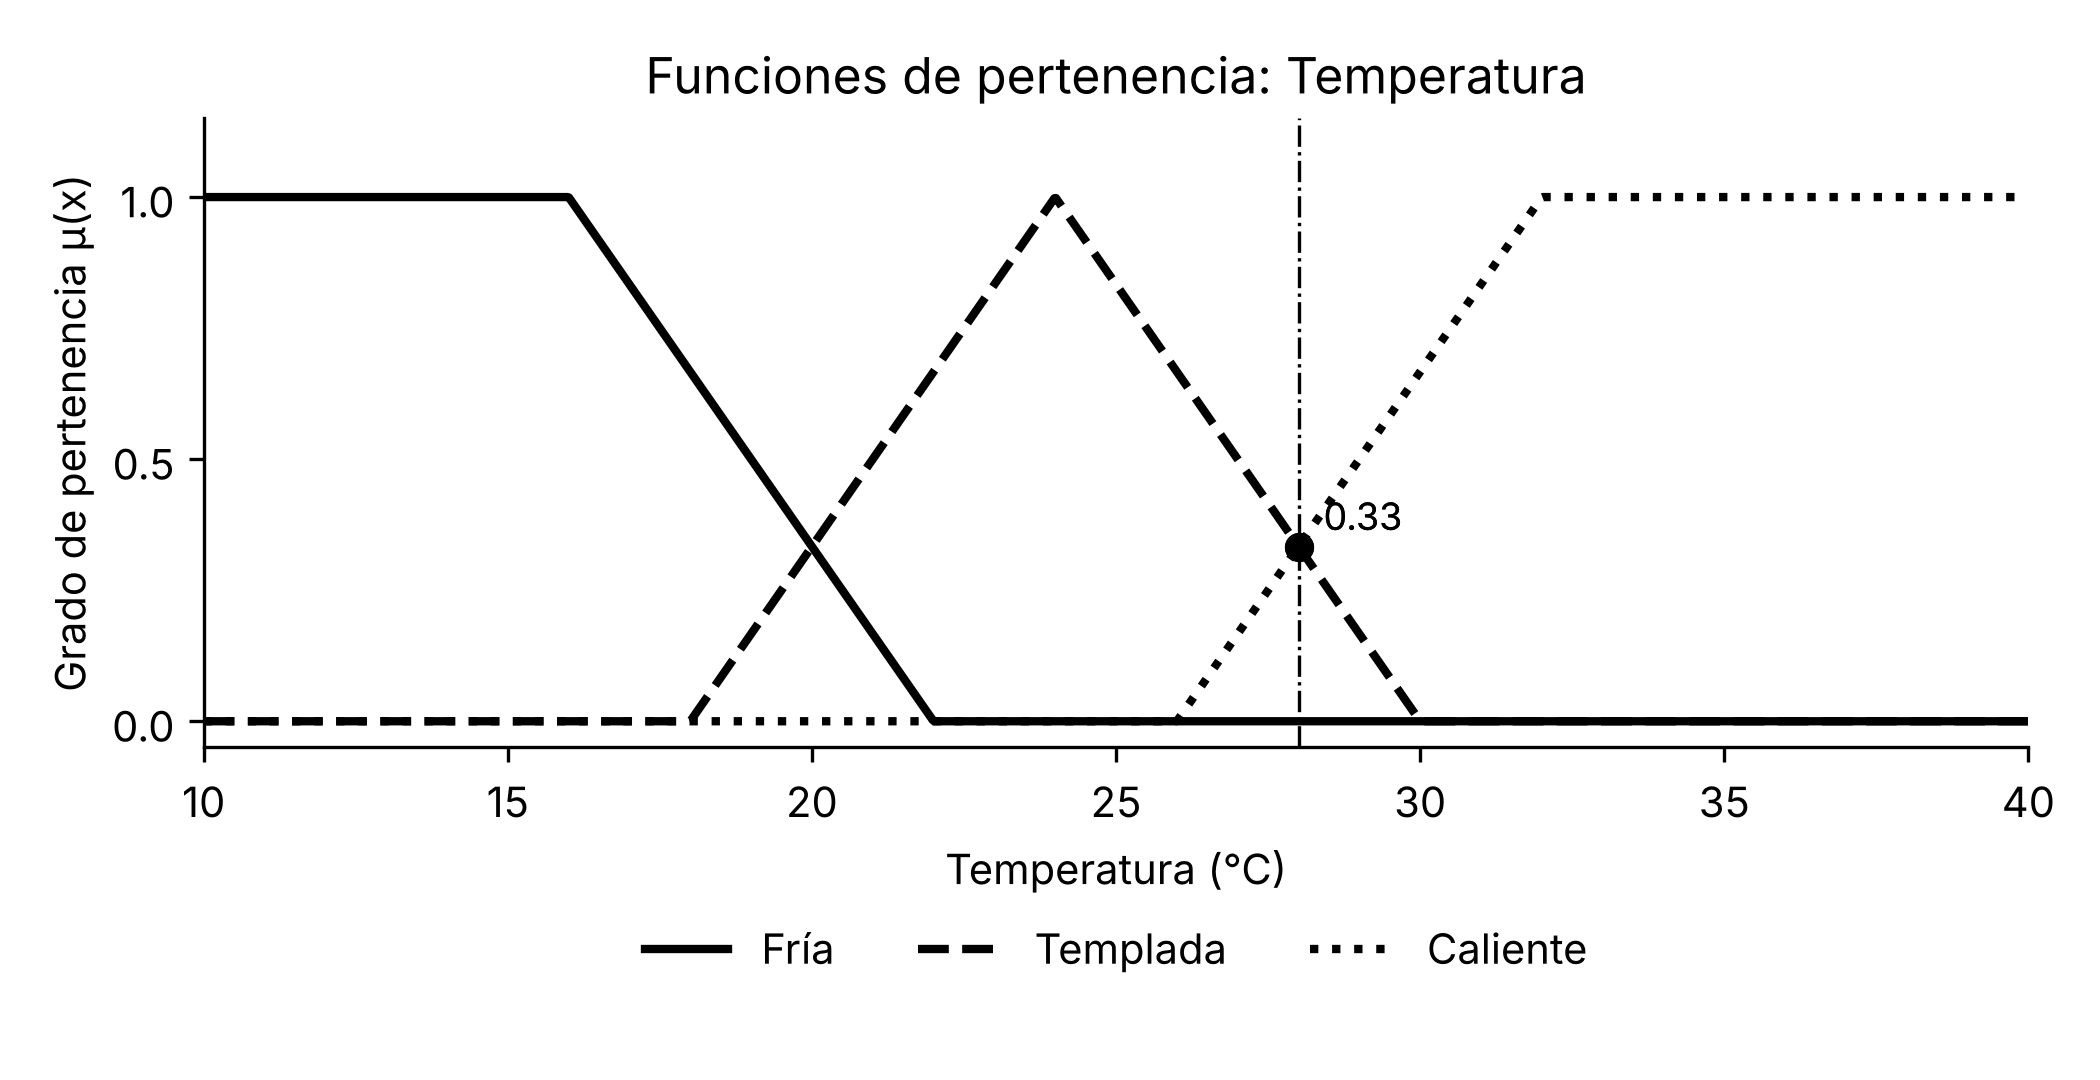
\includegraphics[width=0.7\textwidth]{fig_temperatura.png}\par
\small Figura 1. Funciones de pertenencia de la temperatura.
\end{minipage}

\vspace{1em}

\begin{minipage}{\textwidth}
\centering
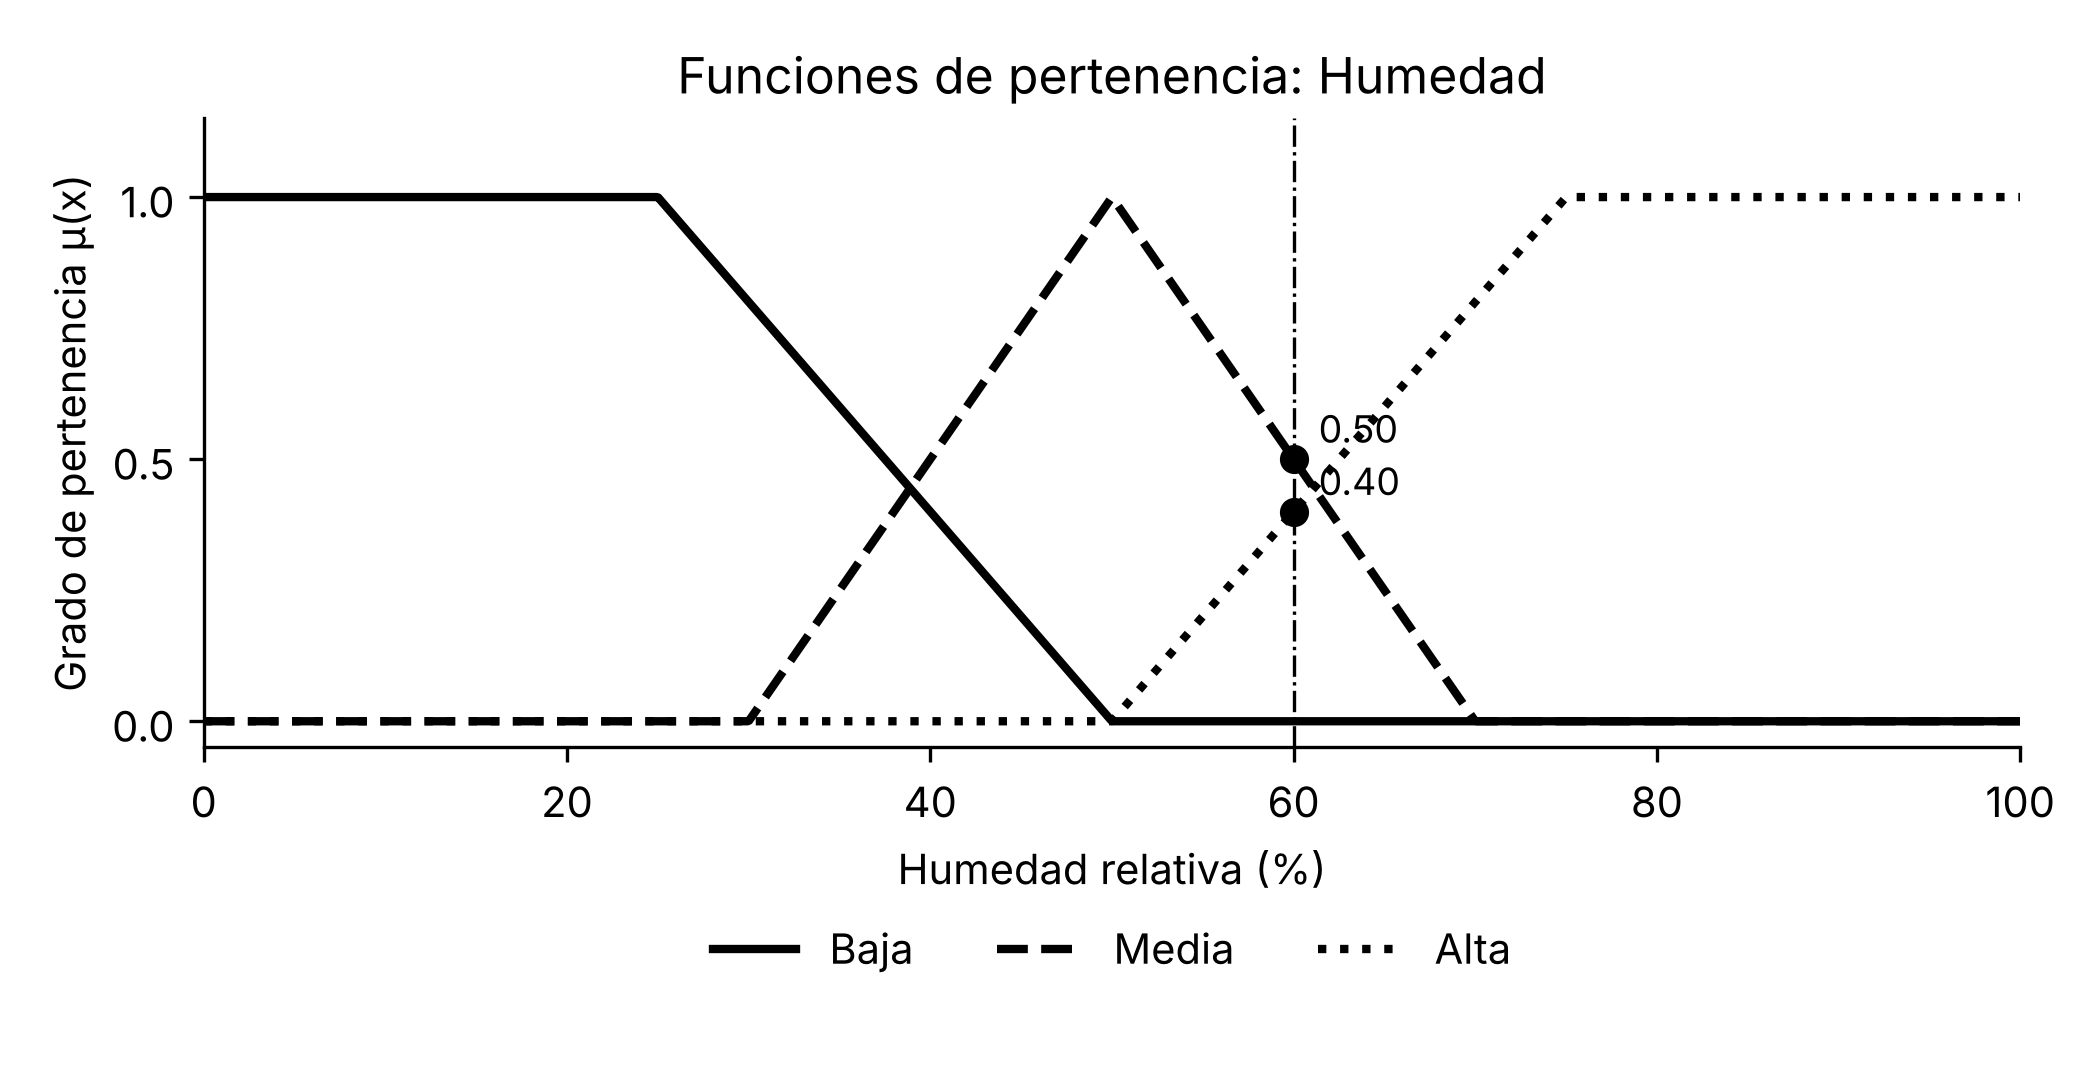
\includegraphics[width=0.7\textwidth]{fig_humedad.png}\par
\small Figura 2. Funciones de pertenencia de la humedad relativa.
\end{minipage}

\vspace{1em}

\begin{minipage}{\textwidth}
\centering
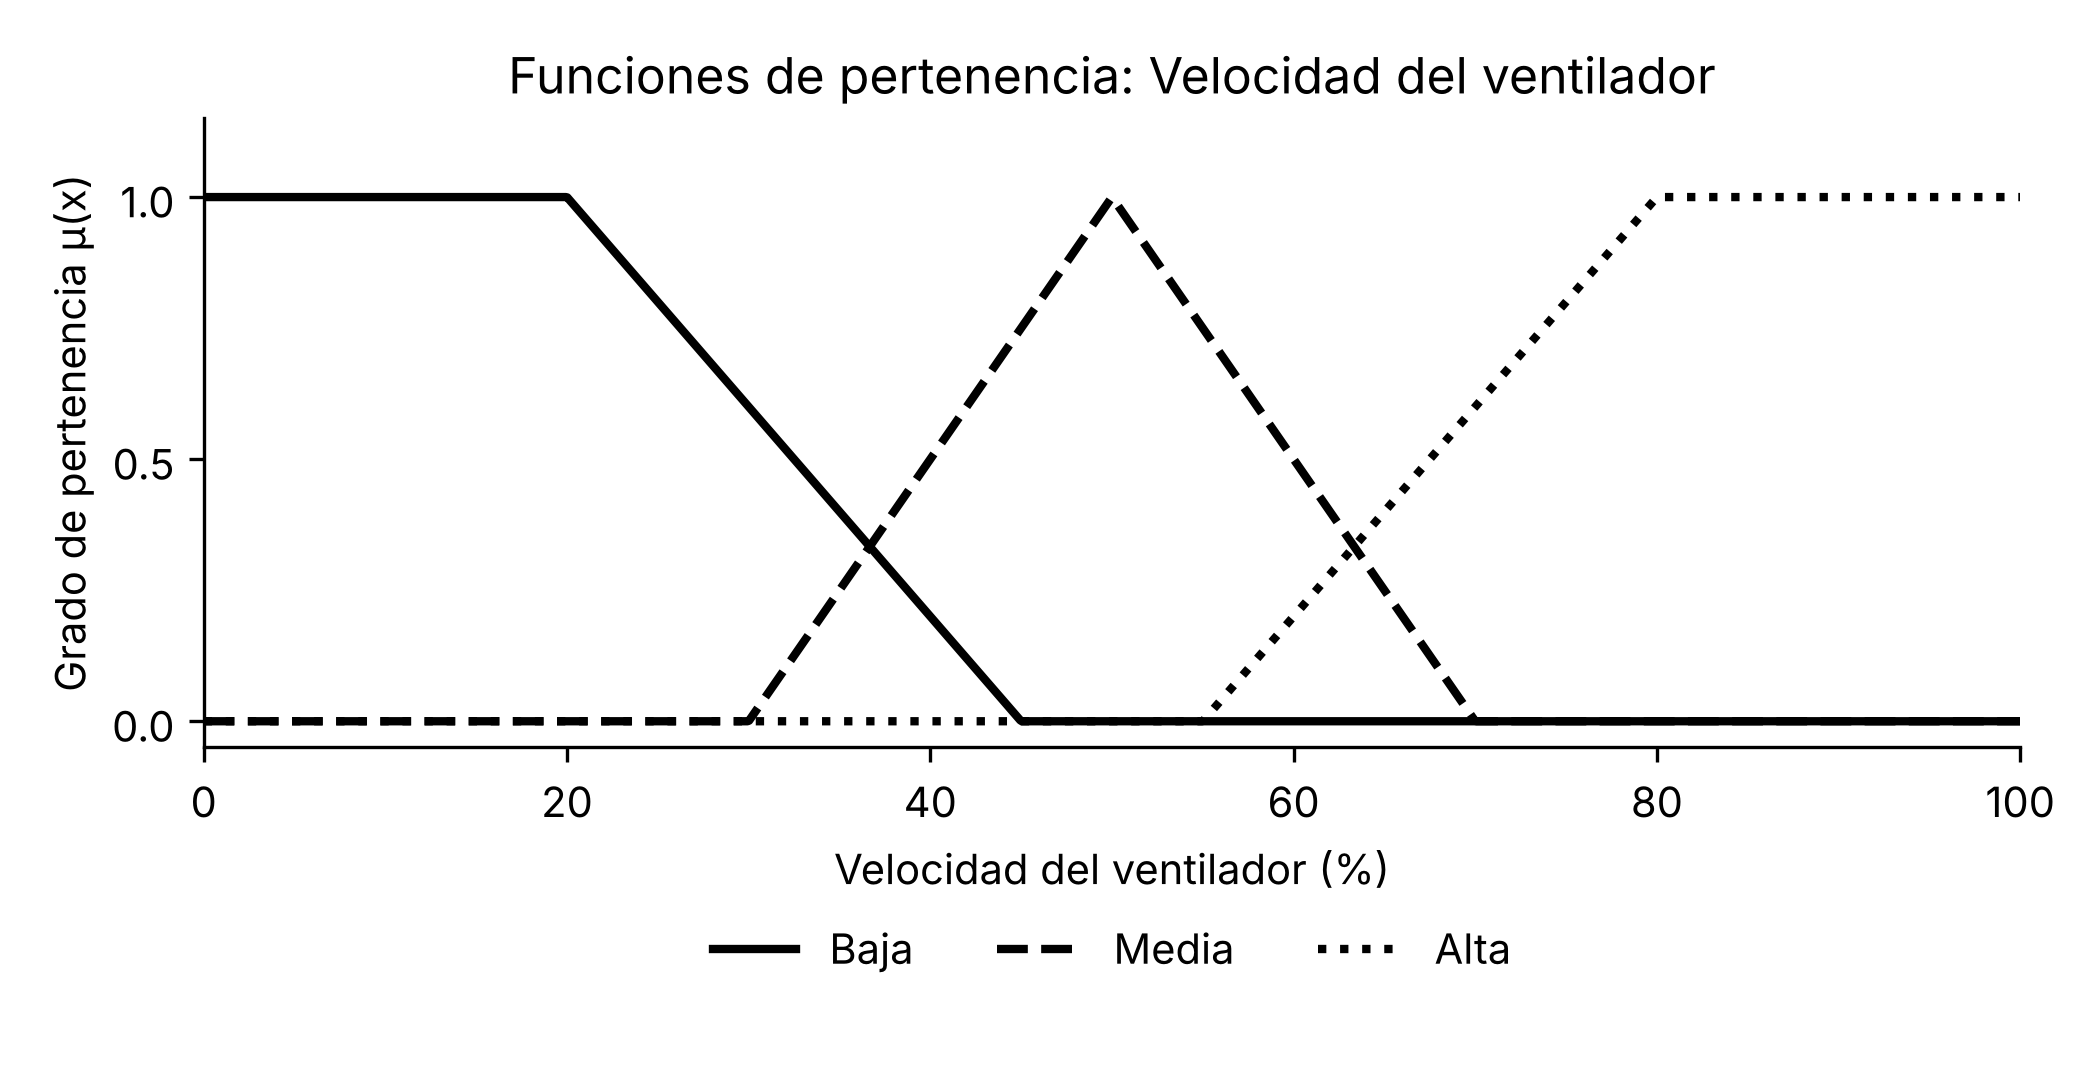
\includegraphics[width=0.7\textwidth]{fig_velocidad.png}\par
\small Figura 3. Funciones de pertenencia de la velocidad del ventilador (variable de salida).
\end{minipage}
\end{center}

\subsection{Fuzzificación}

La fuzzificación es el primer paso del algoritmo de control difuso. Consiste en tomar cada variable de entrada \emph{crisp}, medida por los sensores, y evaluarla en las funciones de pertenencia de sus conjuntos lingüísticos para obtener grados de pertenencia en el intervalo $[0, 1]$. A diferencia de un sistema clásico, donde un valor pertenece o no pertenece a un conjunto, aquí un mismo valor puede pertenecer parcialmente a varios conjuntos a la vez.

Por ejemplo, para una temperatura de $28\,^\circ$C y una humedad de $60\,\%$:
\begin{align*}
\mu_{\text{Fría}}(28) &= 0, &
\mu_{\text{Templada}}(28) &= \frac{30 - 28}{30 - 24} = 0.33, &
\mu_{\text{Caliente}}(28) &= \frac{28 - 26}{32 - 26} = 0.33, \\[6pt]
\mu_{\text{Baja}}(60) &= 0, &
\mu_{\text{Media}}(60) &= \frac{70 - 60}{70 - 50} = 0.50, &
\mu_{\text{Alta}}(60) &= \frac{60 - 50}{75 - 50} = 0.40.
\end{align*}

Estos grados de pertenencia son los valores que se usan como entrada en las cláusulas de Horn de la base de reglas.

\subsection{Justificación de los conjuntos elegidos}

\begin{enumerate}
  \item \textbf{Tres conjuntos por variable.} Son suficientes para describir el problema con términos que una persona usaría de forma natural (fría, templada, caliente) y mantienen la base de reglas manejable: con dos entradas de tres conjuntos cada una resultan 9 combinaciones.
  \item \textbf{Formas triangulares y trapezoidales.} Son simples de calcular y de interpretar, y su costo computacional es bajo, lo que las hace adecuadas para un controlador sencillo.
  \item \textbf{Conjuntos de los extremos con forma de trapecio.} Permiten que los valores extremos tengan pertenencia plena. Por ejemplo, cualquier temperatura menor o igual a $16\,^\circ$C es completamente fría.
  \item \textbf{Traslapes entre conjuntos vecinos.} Los conjuntos se superponen parcialmente (por ejemplo, entre $18$ y $22\,^\circ$C se es a la vez algo fría y algo templada), lo que hace que la transición entre estados sea gradual y que la velocidad del ventilador no cambie bruscamente.
  \item \textbf{Universos del discurso.} El rango de temperatura de $10$ a $40\,^\circ$C abarca las condiciones ambientales habituales en las que se usaría un ventilador. La humedad relativa se define en su rango natural de $0$ a $100\,\%$. La velocidad se expresa como porcentaje de la velocidad máxima para que el modelo no dependa de un ventilador en particular.
\end{enumerate}

% ============================================================
% SECCIONES PENDIENTES (estructura preparada por la Persona 1)
% Cada persona pega su parte debajo del título correspondiente.
% ============================================================

\section{Base de reglas}
\label{sec:reglas}
% Persona 3: base de reglas SI-ENTONCES con operadores de Zadeh
% (min, max, NOT), tabla de reglas y justificación de cada regla.

\section{Caso numérico resuelto a mano}
% Persona 4: antecedentes, implicación, agregación y centroide,
% con la explicación paso a paso del cálculo.

\section{Simulación y análisis de resultados}
% Persona 5: simulación con 3 a 4 casos de prueba, comparación con
% el cálculo manual y comparación contra un sistema clásico con
% umbrales fijos.

\section{Conclusiones y recomendaciones}
% Pendiente de asignar. La tarea pide incluir recomendaciones o
% conclusiones.

% ============================================================
% REFERENCIAS (Persona 1). Se pueden agregar más con \bibitem.
% ============================================================
\begin{thebibliography}{9}
\addcontentsline{toc}{section}{\refname}

\bibitem{zadeh1965}
Zadeh, L. A. (1965). Fuzzy sets. \emph{Information and Control}, 8(3), 338--353.

\bibitem{mamdani1975}
Mamdani, E. H. y Assilian, S. (1975). An experiment in linguistic synthesis with a fuzzy logic controller. \emph{International Journal of Man-Machine Studies}, 7(1), 1--13.

\end{thebibliography}

\end{document}
